\chapter{Implementation of the SENTINEL Automation Fleet}

\section*{Introduction}
\addcontentsline{toc}{section}{Introduction}

This chapter documents the concrete implementation of the three SENTINEL agents. The conceptual design, architectural contract, and UML specification for the Fleet are established in Chapter 3 \S{}3.5 and \S{}3.8, and the technology selection rationale is covered in Chapter 2 \S{}2.4.2. This chapter does not revisit that material. Every section here focuses exclusively on what was built: the actual Python source code, the Power Automate flow step sequences, the exact input file schemas consumed by Agent 3, the real execution logs produced during validation runs, and the platform interfaces through which the system is operated.

The project is developed in a single Visual Studio Code workspace named PFE. The Agents/With Exchange Lib directory contains the four Python files that constitute the entire SENTINEL implementation: email\_listener.py (the shared polling daemon), updatePOI.py (Agent 1), updateretour.py (Agent 2), and updating.py (Agent 3). Configuration is externalised to config/.env. The platform/ directory holds the Angular and Spring Boot codebases for the Unified Platform described in Chapter 6.

\section{Shared Infrastructure: Exchange Connection and Email Listener}

\subsection{Adopted Technology Stack}

The hybrid Python and Power Automate architecture was selected after two failed PoC generations (see Chapter 2 \S{}2.4.2). Table 4.1 records the confirmed implementation choices and the precise technical reason each was retained in the production stack.

\begin{table}[H]
  \centering
  \caption{Adopted technology stack: component, selection, and implementation rationale}
  \renewcommand{\arraystretch}{1.0}
  \begin{tabularx}{\textwidth}{|X|X|X|}
    \hline
    \textbf{Component} & \textbf{Selected Technology} & \textbf{Rationale} \\ \hline
    Exchange access & exchangelib (EWS/NTLM) & Direct protocol-level access; no browser dependency; supports folder navigation, time filtering, and mark-as-read \\ \hline
    Agent logic & Python 3.10 & Full regex, error handling, retry logic; compatible with FastAPI layer and Agent 3 data pipeline \\ \hline
    API layer & FastAPI + Uvicorn & Async background tasks; UUID job store; native file upload; clean Spring Boot integration \\ \hline
    Server-side ops & Power Automate Cloud & Handles SharePoint + Planner + Azure AD without OAuth token management in Python \\ \hline
    Proxy management & Corporate proxy + NO\_PROXY & Exchange via proxyparfil:8080; Power Automate bypassed via NO\_PROXY to avoid HTTP 403 URLBlocked \\ \hline
  \end{tabularx}
\end{table}

The global SENTINEL Fleet architecture implementing this stack is shown in Figure 4.1. The three agents share the same FastAPI execution layer, which proxies all Exchange interactions while delegating all SharePoint and Planner operations to Power Automate flows.

\begin{figure}[H]
  \centering
  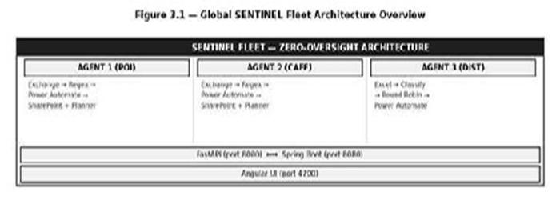
\includegraphics[width=0.52\textwidth,max width=\textwidth]{images/image36.png}
  \caption{Global SENTINEL Fleet Architecture Overview}
  \label{fig:image36}
\end{figure}

\subsection{The Email Listener Daemon}

The email\_listener.py module is the entry point for the event-driven agents. It runs a polling loop at a 60-second interval, connects to the Orange Exchange server over EWS/NTLM, checks both monitored folders simultaneously, and dispatches the appropriate agent script as a subprocess when a new unread email is detected. The routing contract is declared in the startup banner: FINOI (POI) triggers updatePOI.py, and \_retour CAFF GEDAFFAIRES triggers updateretour.py.

\begin{figure}[H]
  \centering
  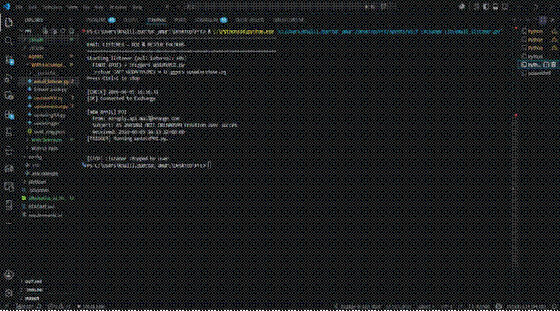
\includegraphics[width=0.52\textwidth,max width=\textwidth]{images/image37.png}
  \caption{Email Listener Live Execution: New POI Email Detected and Agent 1 Triggered}
  \label{fig:image37}
\end{figure}

\begin{center}\small\textbf{Listing: Email listener core polling loop (email\_listener.py)}\end{center}
\begin{Verbatim}[breaklines=true,fontsize=\footnotesize,frame=single]
credentials = Credentials(USERNAME, PASSWORD) config = Configuration(
service_endpoint=EWS_URL,
credentials=credentials,
auth_type=NTLM,
retry_policy=FaultTolerance(max_wait=60) ) account = Account(MAILBOX, config=config, access_type=DELEGATE)
while True:
finoi = account.inbox / "Dossier AGILIS" / "FINOI"
new_poi = list(finoi.filter(is_read=False)
.order_by("-datetime_received")[:1])
if new_poi:
subprocess.run(["python", "updatePOI.py"])
caff = account.inbox / "_retour CAFF GEDAFFAIRES"
new_caff = list(caff.filter(is_read=False)
.order_by("-datetime_received")[:1])
if new_caff:
subprocess.run(["python", "updateretour.py"])
time.sleep(POLL_INTERVAL)
\end{Verbatim}

\subsection{Exchange Connection: NTLM, Proxy, and SSL Configuration}

All three agents instantiate the same Exchange connection pattern. The corporate proxy (proxyparfil.si.fr.intraorange:8080) is required for EWS traffic. Power Automate webhook calls must bypass it routing them through the proxy returns HTTP 403 URLBlocked which is resolved by setting NO\_PROXY=powerplatform.com. Orange Exchange uses a self-signed certificate, handled by a custom NoVerifyHTTPAdapter.

\begin{table}[H]
  \centering
  \caption{Five-stage execution skeleton shared by Agents 1 and 2}
  \renewcommand{\arraystretch}{1.0}
  \begin{tabularx}{\textwidth}{|>{\raggedright\arraybackslash}p{2.3cm}|X|X|}
    \hline
    \textbf{Stage} & \textbf{Action} & \textbf{Implementation Detail} \\ \hline
    1 & Exchange connection & exchangelib connects to exchange.itn.intraorange via EWS with NTLM; NoVerifyHTTPAdapter for self-signed SSL; delegate access on shared mailbox \\ \hline
    2 & Folder navigation & account.inbox / "Dossier AGILIS" / "FINOI" for Agent 1; account.inbox / "\_retour CAFF GEDAFFAIRES" for Agent 2 \\ \hline
    3 & Field extraction & Regex on subject + body; mandatory fields extracted; missing fields escalate to log; extracted fields serialised to Python dict \\ \hline
    4 & Webhook trigger & requests.post to signed Power Automate flow URL; NO\_PROXY bypass; HTTP 200/202 confirms flow instantiation \\ \hline
    5 & Mark-as-read + exit & item.is\_read = True; item.save(); agent exits; log captured by FastAPI job store \\ \hline
  \end{tabularx}
\end{table}

\begin{center}\small\textbf{Listing: Exchange connection setup: NTLM, NoVerifyHTTPAdapter, proxy (shared by all agents)}\end{center}
\begin{Verbatim}[breaklines=true,fontsize=\footnotesize,frame=single]
os.environ["HTTP_PROXY"]
= "http://proxyparfil.si.fr.intraorange:8080" os.environ["HTTPS_PROXY"] = "http://proxyparfil.si.fr.intraorange:8080" os.environ["NO_PROXY"]	= "powerplatform.com"
urllib3.disable_warnings(urllib3.exceptions.InsecureRequestWarning)
class NoVerifyHTTPAdapter(requests.adapters.HTTPAdapter):
def send(self, *args, **kwargs):
kwargs["verify"] = False
return super().send(*args, **kwargs)
session = requests.Session() session.mount("https://", NoVerifyHTTPAdapter())
config = Configuration(
service_endpoint=EWS_URL, credentials=Credentials(USERNAME, PASSWORD),
auth_type=NTLM, retry_policy=FaultTolerance(max_wait=60) ) account = Account(MAILBOX, config=config, access_type=DELEGATE)
\end{Verbatim}

\begin{table}[H]
  \centering
  \caption{Cross-cutting operational concerns: credentials, proxy, SSL, logging, error handling}
  \renewcommand{\arraystretch}{1.0}
  \begin{tabularx}{\textwidth}{|X|X|}
    \hline
    \textbf{Concern} & \textbf{Implementation} \\ \hline
    Credentials & EWS\_URL, USERNAME, PASSWORD, MAILBOX defined as module constants; externalised to .env via python-dotenv, excluded from version control \\ \hline
    Proxy configuration & HTTP\_PROXY and HTTPS\_PROXY set to proxyparfil.si.fr.intraorange:8080; NO\_PROXY set to powerplatform.com for direct Power Automate calls without HTTP 403 URLBlocked \\ \hline
    SSL & IGNORE\_SSL disables certificate verification via NoVerifyHTTPAdapter; urllib3 InsecureRequestWarning suppressed \\ \hline
    Logging & stdout captured by FastAPI redirect\_stdout into StringIO buffer; stored as list in job record; accessible via /api/jobs/\{id\} \\ \hline
    Error handling & try/except around all major phases; RuntimeError for terminal conditions; traceback printed to captured buffer \\ \hline
    Retry policy & FaultTolerance(max\_wait=60) passed to exchangelib Configuration; handles transient Exchange connectivity failures \\ \hline
  \end{tabularx}
\end{table}

\section{Agent 1: POI Validation Implementation}

Agent 1 (updatePOI.py) targets the FINOI folder. Its deployment topology is shown in Figure 4.3: the FastAPI server receives the trigger from the email listener or from the Unified Platform, navigates to account.inbox / "Dossier AGILIS" / "FINOI", applies the extraction engine, and fires the Power Automate POI flow which autonomously updates SUIVI and creates the Planner task.

\begin{figure}[H]
  \centering
  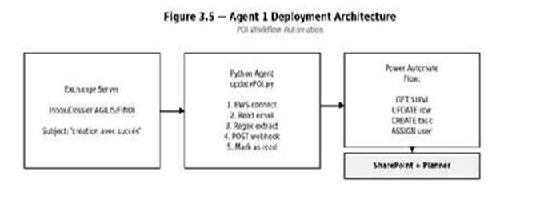
\includegraphics[width=0.52\textwidth,max width=\textwidth]{images/image38.png}
  \caption{Agent 1 Deployment Architecture}
  \label{fig:image38}
\end{figure}

\subsection{Folder Navigation and Email Selection}

Emails are retrieved in reverse chronological order. Each email is checked against two conditions: the subject must contain "création avec succès" (confirming it is a successful POI creation notification) and the string "OEIE" (confirming it carries the required identifiers). Emails with type\_demande\_POI containing the word "anticipation" are explicitly skipped, as they represent pre-notifications not yet subject to validation. Non-matching emails are logged with [SKIP] and do not halt processing of the remaining batch.

\begin{center}\small\textbf{Listing: Agent 1 folder navigation and email selection (updatePOI.py)}\end{center}
\begin{Verbatim}[breaklines=true,fontsize=\footnotesize,frame=single]
folder = account.inbox / "Dossier AGILIS" / "FINOI" emails = list(folder.all().order_by("-datetime_received")) print(f"[OK] Folder resolved: {len(emails)} emails")
for item in emails:
subject = item.subject or ""
body
= item.text_body or item.body or ""
if "creation avec succes" not in subject.lower():
continue
print(f"[CHECKING] Subject: '{subject}'")
print(f"	[OK] This is a creation success email. Processing...")
print(f"	[INFO] {len(body)} chars
\end{Verbatim}

\subsection{Six-Field Regex Extraction Engine}

The extraction engine applies six independent regex patterns to the email body. A critical bug was discovered and fixed during development: the initial PC pattern used \textbackslash{}\textbackslash{}d+ which silently truncated alphanumeric codes such as DP0610012500255 to DP06100125002 at the first non-digit character. The corrected pattern uses [\textasciicircum{}\#\textbackslash{}\textbackslash{}s]+ to capture any character sequence up to the Agilis hash delimiter. Table 4.4 documents all six patterns.

\begin{table}[H]
  \centering
  \caption{Agent 1 six-field extraction patterns with implementation notes}
  \renewcommand{\arraystretch}{1.0}
  \footnotesize
  \begin{tabularx}{\textwidth}{|X|X|X|X|X|}
    \hline
    \textbf{Field} & \textbf{Regex Pattern} & \textbf{Implementation Note} & \textbf{} & \textbf{} \\ \hline
    AS & AS\textbackslash{}\textbackslash{}s\textit{n[\textdegree{}o]?\textbackslash{}\textbackslash{}s}(\textbackslash{}\textbackslash{}d+) & Handles Agilis variants: "AS n\textdegree{}2604377", "AS no2604377", "AS 2604377" &  &  \\ \hline
    OEIE & OEIE\textbackslash{}\textbackslash{}s\textit{n[\textdegree{}o]?\textbackslash{}\textbackslash{}s}([A-Z0-9]+) & Captures alphanumeric codes: ALM600681, SBA600840, ORL600599 &  &  \\ \hline
    Affaire & AFFAIRE\textbackslash{}\textbackslash{}s+([A-Z0-9]+) & Applied to email body text &  &  \\ \hline
    Etablissement & compte de l.établissement\textbackslash{}\textbackslash{}s+(.+?)[.\textbackslash{}\textbackslash{}n] & Extracts site name up to period or newline boundary &  &  \\ \hline
    PC & **((PC & PA & DP)[\textasciicircum{}\#\textbackslash{}\textbackslash{}s]+)\#** & Critical fix: initial \textbackslash{}\textbackslash{}d+ silently truncated alphanumeric codes (e.g. DP0610012500255). Corrected to [\textasciicircum{}\#\textbackslash{}\textbackslash{}s]+ to capture full code up to hash delimiter. \\ \hline
    type\_demande\_POI & **(?:PC & PA & DP)[\textasciicircum{}\#\textbackslash{}\textbackslash{}s]+\#([\textasciicircum{}\#]+)\#** & Captures string between first and second \# delimiter in Commentaire AS \\ \hline
  \end{tabularx}
\end{table}

\begin{center}\small\textbf{Listing: Regex extraction and mandatory field validation (updatePOI.py)}\end{center}
\begin{Verbatim}[breaklines=true,fontsize=\footnotesize,frame=single]
patterns = {
"AS":
r"AS\\s*n[o]?\\s*(\\d+)",
"OEIE":
r"OEIE\\s*n[o]?\\s*([A-Z0-9]+)",
"Affaire":
r"AFFAIRE\\s+([A-Z0-9]+)",
"Etablissement":
r"compte de l.etablissement\\s+(.+?)[.\\n]",
"PC":
r"((PC
\end{Verbatim}

\subsection{Execution Log: Agent 1 on Live Exchange Data}

\begin{figure}[H]
  \centering
  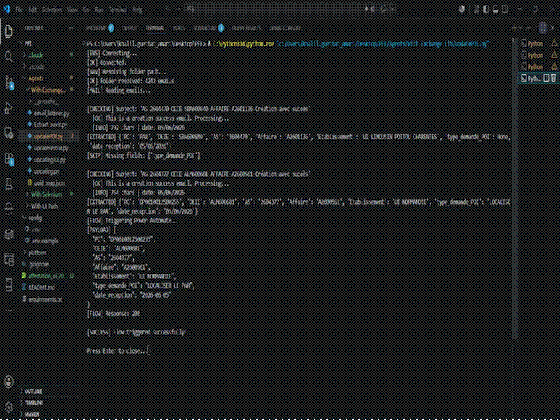
\includegraphics[width=0.52\textwidth,max width=\textwidth]{images/image39.png}
  \caption{Agent 1 Execution Log: Field Extraction, Skip Decision, and Successful Flow Dispatch}
  \label{fig:image39}
\end{figure}

\subsection{Power Automate Orchestration Flow}

Once all mandatory fields pass validation, the agent dispatches a seven-field JSON payload to the signed Power Automate flow URL. The flow executes seven server-side steps autonomously, resolving the responsible Agent Traitant via Azure AD lookup without any further agent involvement.

\begin{table}[H]
  \centering
  \caption{Agent 1 Power Automate flow: seven-step execution sequence}
  \renewcommand{\arraystretch}{1.0}
  \begin{tabularx}{\textwidth}{|>{\raggedright\arraybackslash}p{2.3cm}|X|}
    \hline
    \textbf{Step} & \textbf{Action} \\ \hline
    1 & HTTP request trigger flow instantiated by Python POST; body schema declares PC, OEIE, AS, Affaire, Etablissement, type\_demande\_POI, date\_reception \\ \hline
    2 & Get items SharePoint filter SUIVI by OData: REF\_AU eq "\textless{}PC\textgreater{}"; cardinality must be exactly one \\ \hline
    3 & Read PF and Agent Traitant from the matching SUIVI row \\ \hline
    4 & Update item set Ref\_POI\_PAR\_1 = OEIE and Date\_de\_creation\_POI = date\_reception \\ \hline
    5 & Create task in POI alerte Planner bucket; title = "POI \textless{}OEIE\textgreater{}" \\ \hline
    6 & Update task notes: PF / PC / AS-OEIE-POI / Etablissement / SUIVI deep link \\ \hline
    7 & Assign task via Azure AD lookup of the user whose display name matches Agent\_Traitant \\ \hline
  \end{tabularx}
\end{table}

\begin{figure}[H]
  \centering
  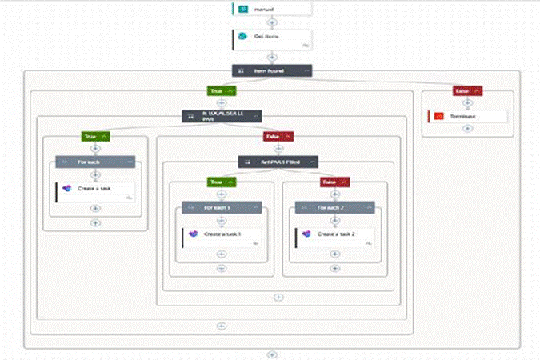
\includegraphics[width=0.52\textwidth,max width=\textwidth]{images/image40.png}
  \caption{Agent 1 Power Automate Flow Logic}
  \label{fig:image40}
\end{figure}

\begin{center}\small\textbf{Listing: Power Automate webhook dispatch with NO\_PROXY bypass (updatePOI.py)}\end{center}
\begin{Verbatim}[breaklines=true,fontsize=\footnotesize,frame=single]
payload = {
"PC": extracted["PC"], "OEIE": extracted["OEIE"],
"AS": extracted["AS"], "Affaire": extracted["Affaire"],
"Etablissement": extracted["Etablissement"],
"type_demande_POI": extracted["type_demande_POI"],
"date_reception": extracted["date_reception"], } print(f"[PAYLOAD] {json.dumps(payload, indent=2, ensure_ascii=False)}")
# NO_PROXY set at module load webhook bypasses corporate proxy response = requests.post(FLOW_URL, json=payload, verify=False) print(f"[FLOW] Response: {response.status_code}")
if response.status_code in (200, 202):
item.is_read = True
item.save()
print("[SUCCESS] Flow triggered successfully!")
\end{Verbatim}

The Planner task output produced by the flow is shown in Figure 4.6. The task is created in the POI alerte bucket, titled with the OEIE code, assigned to the Agent Traitant resolved from SUIVI, and annotated with PF, PC, AS, Etablissement, and a SUIVI deep link in its notes.

\begin{figure}[H]
  \centering
  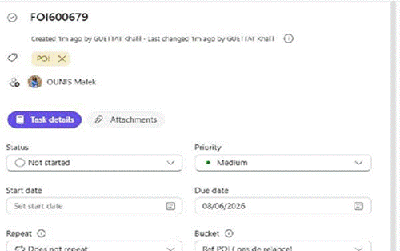
\includegraphics[width=0.52\textwidth,max width=\textwidth]{images/image41.png}
  \caption{Planner Task Output Created by Agent 1}
  \label{fig:image41}
\end{figure}

\subsection{Platform Control Interface}

Agent 1 is accessible through the Guichet OI Automation Platform (Figure 4.7). The Email Listener toggle activates the 60-second polling daemon; the Run Agent Manually card triggers a single on-demand execution. This dual-mode design was validated with the SDM as providing the correct balance between fully automated monitoring and controlled on-demand execution without command-line access.

\begin{figure}[H]
  \centering
  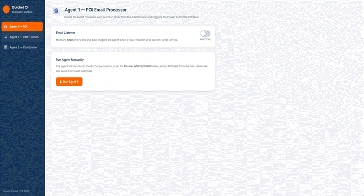
\includegraphics[width=0.52\textwidth,max width=\textwidth]{images/image42.png}
  \caption{Unified Platform: Agent 1 POI Email Processor Control Page}
  \label{fig:image42}
\end{figure}

\section{Agent 2: CAFF Returns Implementation}

Agent 2 (updateretour.py) targets the \_retour CAFF GEDAFFAIRES folder. Table 4.6 documents the three operational failure modes that the agent was designed to eliminate. Figure 4.8 shows the deployment architecture.

\begin{table}[H]
  \centering
  \caption{Pre-automation CAFF return failure modes eliminated by Agent 2}
  \renewcommand{\arraystretch}{1.0}
  \begin{tabularx}{\textwidth}{|X|X|}
    \hline
    \textbf{Failure Mode} & \textbf{Operational Impact} \\ \hline
    Missed returns & Return arriving after 5 PM not picked up until next morning; one-day KPI budget already half-consumed before anyone acts \\ \hline
    Delayed assignments & Responsible Agent Traitant not immediately identifiable; inbox monitor must open SUIVI, look up PC, then forward via Teams \\ \hline
    Untracked treatments & No Planner task created even when handoff happened fast; no open-work item drives consultant planning or Pilot weekly review \\ \hline
  \end{tabularx}
\end{table}

\begin{figure}[H]
  \centering
  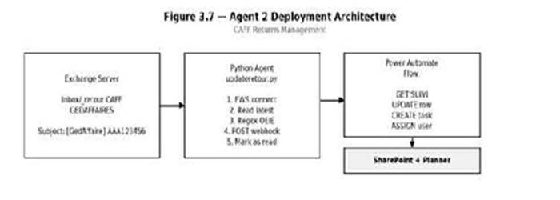
\includegraphics[width=0.52\textwidth,max width=\textwidth]{images/image43.png}
  \caption{Agent 2 Deployment Architecture}
  \label{fig:image43}
\end{figure}

\subsection{Single-Pattern OEIE Extraction}

Agent 2 applies a single strict regex pattern to the subject line: \textbackslash{}\textbackslash{}b([A-Z]\{3\}\textbackslash{}\textbackslash{}d\{6\})\textbackslash{}\textbackslash{}b, matching exactly three uppercase letters followed by exactly six digits. GedAffaire push mails use this format consistently. A subject such as "TR: [GedAffaire] : CAFF 22 Cochard Claire dossier SBR502867" yields OEIE: SBR502867 immediately. If the pattern produces no match, Agent 2 raises RuntimeError and terminates unlike Agent 1, there is no fallback iteration, because a non-matching subject indicates a structurally unexpected email requiring human escalation.

\begin{center}\small\textbf{Listing: Agent 2 OEIE extraction with hard-fail on no-match (updateretour.py)}\end{center}
\begin{Verbatim}[breaklines=true,fontsize=\footnotesize,frame=single]
folder = account.inbox / "_retour CAFF GEDAFFAIRES" emails = list(folder.filter(is_read=False)
.order_by("-datetime_received")) print(f"[OK] {len(emails)} emails found")
if not emails:
print("[INFO] No unread CAFF emails. Exiting.")
sys.exit(0)
item	= emails[0]
# process only the most recent subject = item.subject or "" print(f"[INFO] Subject: {subject}")
match = re.search(r"\\b([A-Z]{3}\\d{6})\\b", subject) if not match:
raise RuntimeError(f"OEIE pattern not found: '{subject}'")
oeie = match.group(1) print(f"[EXTRACTED] OEIE: {oeie}")
response = requests.post(CAFF_FLOW_URL, json={"OEIE": oeie}, verify=False) print(f"[PAYLOAD] {{\"OEIE\": \"{oeie}\"}}") print(f"[FLOW] Response: {response.status_code}")
if response.status_code in (200, 202):
item.is_read = True ; item.save()
print(f"[SUCCESS] OEIE '{oeie}' sent to flow")
\end{Verbatim}

\subsection{Execution Log: Agent 2 on Live Exchange Data}

Figure 4.9 shows Agent 2 processing a live CAFF return. The folder contains 247 unread emails. The agent reads the most recent, extracts OEIE SBR502867 from the subject "TR: [GedAffaire] : CAFF 22 Cochard Claire dossier SBR502867", dispatches \{"OEIE": "SBR502867"\} to Power Automate, receives HTTP 202, marks the email as read, and terminates in under 8 seconds.

\begin{figure}[H]
  \centering
  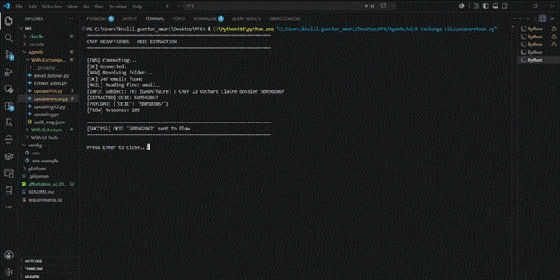
\includegraphics[width=0.52\textwidth,max width=\textwidth]{images/image44.png}
  \caption{Agent 2 Execution Log: OEIE Extraction and Atomic Flow Dispatch}
  \label{fig:image44}
\end{figure}

\subsection{Power Automate Orchestration Flow and Notification}

\begin{figure}[H]
  \centering
  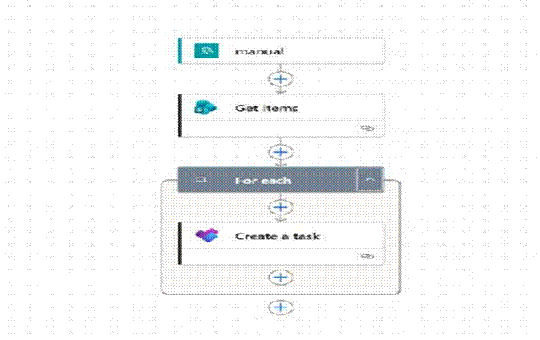
\includegraphics[width=0.52\textwidth,max width=\textwidth]{images/image45.png}
  \caption{Agent 2 Power Automate Flow Logic}
  \label{fig:image45}
\end{figure}

On completion of the Power Automate flow, the assigned consultant receives an immediate Planner assignment notification (Figure 4.11). This notification closes the routing gap the consultant learns of the CAFF return within seconds of its arrival in the shared mailbox, regardless of the time of day.

\begin{figure}[H]
  \centering
  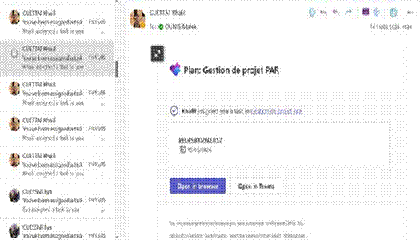
\includegraphics[width=0.52\textwidth,max width=\textwidth]{images/image46.png}
  \caption{Consultant Notification Email Generated by Agents}
  \label{fig:image46}
\end{figure}

\subsection{Platform Control Interface}

\begin{figure}[H]
  \centering
  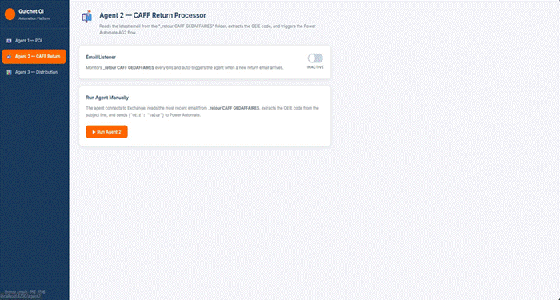
\includegraphics[width=0.52\textwidth,max width=\textwidth]{images/image47.png}
  \caption{Unified Platform: Agent 2 CAFF Return Processor Control Page}
  \label{fig:image47}
\end{figure}

\section{Agent 3: Distribution Engine Implementation}

Agent 3 (updating.py) is architecturally distinct from Agents 1 and 2. Its stimulus is a daily batch of Excel rows, not individual emails. Its deployment architecture, shown in Figure 4.13, reflects this: three files are ingested via the desktop UI, processed through a six-step pandas pipeline, and dispatched as individual Power Automate webhooks.

\begin{figure}[H]
  \centering
  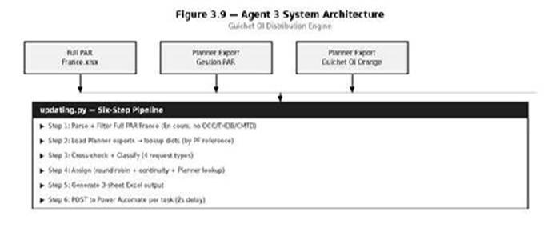
\includegraphics[width=0.52\textwidth,max width=\textwidth]{images/image48.png}
  \caption{Agent 3 System Architecture}
  \label{fig:image48}
\end{figure}

\subsection{Input File Structure}

\begin{table}[H]
  \centering
  \caption{Agent 3 input file schemas and roles}
  \renewcommand{\arraystretch}{1.0}
  \begin{tabularx}{\textwidth}{|X|X|}
    \hline
    \textbf{Input File} & \textbf{Content and Role} \\ \hline
    Full PAR France (.xlsx) & Master dossier inventory from Agilis. Contains code\_unique, ref\_PC, REF\_PAR, raison\_sociale, RIP, code\_insee, date\_validation\_dossier, pc\_di\_demande\_datecreation. Filtered to the most recent injection batch. \\ \hline
    Planner 1 Gestion de Projet PAR (.xlsx) & Planner export in English column format. Provides Task Name (= PC reference), Bucket, Status, Priority, Assigned To. Searched first for consultant lookup. \\ \hline
    Planner 2 Guichet OI Orange (.xlsx) & Planner export in French column format (Nom de tâche, Statut, Priorité, Attribué à). Assigned To values are M365 UUIDs resolved via uuid\_map.json. Searched when Planner 1 yields no match. \\ \hline
  \end{tabularx}
\end{table}

\begin{figure}[H]
  \centering
  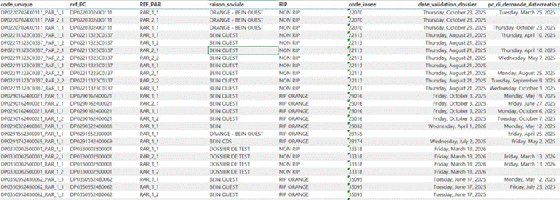
\includegraphics[width=0.52\textwidth,max width=\textwidth]{images/image49.png}
  \caption{Full PAR France Input Workbook: Column Structure and Representative Rows}
  \label{fig:image49}
\end{figure}

\begin{figure}[H]
  \centering
  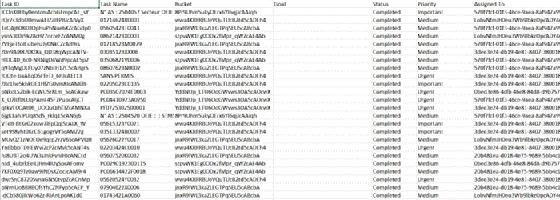
\includegraphics[width=0.52\textwidth,max width=\textwidth]{images/image50.png}
  \caption{Planner 1: Gestion de Projet PAR Export (English Column Format)}
  \label{fig:image50}
\end{figure}

\begin{figure}[H]
  \centering
  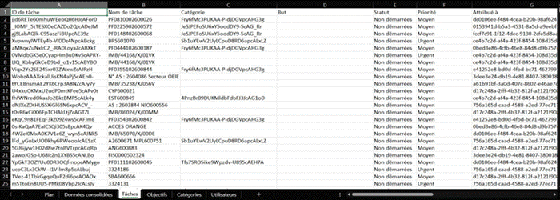
\includegraphics[width=0.52\textwidth,max width=\textwidth]{images/image51.png}
  \caption{Planner 2: Guichet OI Orange Export (French Columns, M365 UUID Assigned To)}
  \label{fig:image51}
\end{figure}

\subsection{Six-Step Pandas Processing Pipeline}

\begin{center}\small\textbf{Listing: Step 1: Full PAR France filtering (updating.py)}\end{center}
\begin{Verbatim}[breaklines=true,fontsize=\footnotesize,frame=single]
df = pd.read_excel(fullpar_path) df = df[df["pc_di_demande_etat"] == "En cours"]
# active only df = df[df["raison_sociale"] != "OCC"]
# exclude OCC mask = df["pc_di_demande_commentaireclient"].str.startswith(
("THDB", "GTHD", "CMTD"), na=False) df = df[~mask] latest = df["pc_di_demande_datecreation"].max() df = df[df["pc_di_demande_datecreation"] == latest] print(f"[STEP 1] {len(df)} rows retained (date: {latest})")
\end{Verbatim}

Step 3 applies the classification rules documented in Table 4.8 to each row.

\begin{table}[H]
  \centering
  \caption{Request type classification rules applied in Step 3}
  \renewcommand{\arraystretch}{1.0}
  \footnotesize
  \begin{tabularx}{\textwidth}{|X|X|X|X|}
    \hline
    \textbf{Type} & \textbf{Condition on type\_demande} & \textbf{Condition on Intervention} & \textbf{Condition on date\_completude} \\ \hline
    RAR & Starts with "RAR" & Any & Any \\ \hline
    Nouvelle Demande & Contains "PAR\_1\_1" & Attente envoie accusé réception & NULL \\ \hline
    Retour Complétude & Starts with "PAR", not PAR\_1\_1 & Any & NULL \\ \hline
    Go Lancement Projet & Starts with "PAR" & PAR CAFF or PAR en ligne & NOT NULL \\ \hline
    Default & All other cases & Any & Any \\ \hline
  \end{tabularx}
\end{table}

\begin{center}\small\textbf{Listing: Step 3: request type classification (updating.py)}\end{center}
\begin{Verbatim}[breaklines=true,fontsize=\footnotesize,frame=single]
def classify_row(row):
ref
= str(row["REF_PAR"]).strip()
intv
= str(row.get("Intervention", "")).strip()
date_c = row.get("date_completude")
if ref.startswith("RAR"):
return "RAR"
if "PAR_1_1" in ref and intv == "Attente envoie accuse reception" \\
and pd.isna(date_c):
return "Nouvelle Demande"
if ref.startswith("PAR") and "PAR_1_1" not in ref and pd.isna(date_c):
return "Retour Completude"
if ref.startswith("PAR") and intv in ("PAR CAFF", "PAR en ligne") \\
and not pd.isna(date_c):
return "Go Lancement Projet"
return "Default"
df["request_type"] = df.apply(classify_row, axis=1)
\end{Verbatim}

\subsection{Round-Robin Routing Algorithm with State Persistence}

Step 4 routes Nouvelle Demande rows using the round-robin algorithm shown in Figure 4.17. The persistent index (last\_assigned) carries across daily runs via the desktop UI dropdown, ensuring fairness accumulates over time rather than resetting to zero each day. Continuity-of-treatment takes priority: any row for a dossier already in progress routes to the existing Agent Traitant regardless of the current round-robin position. Table 4.9 documents the SUIVI lookup outcomes and their routing decisions. Table 4.10 documents the priority and deadline assigned to each request type.

\begin{figure}[H]
  \centering
  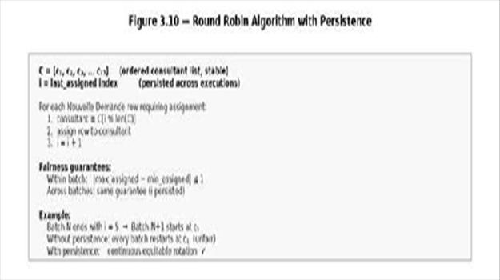
\includegraphics[width=0.52\textwidth,max width=\textwidth]{images/image52.png}
  \caption{Round-Robin Algorithm with Persistent State}
  \label{fig:image52}
\end{figure}

\begin{table}[H]
  \centering
  \caption{SUIVI lookup outcomes and routing decisions}
  \renewcommand{\arraystretch}{1.0}
  \begin{tabularx}{\textwidth}{|X|X|}
    \hline
    \textbf{Lookup Outcome} & \textbf{Routing Decision} \\ \hline
    PF found, non-null Agent Traitant, progress In Progress or Not Started & Route to that consultant continuity of treatment preserved \\ \hline
    PF found, null or invalid Agent Traitant & Edge case falls back to round-robin engine \\ \hline
    PF found, progress Completed, completion date before creation date & New injection falls back to round-robin engine \\ \hline
    PF not found in either Planner & New dossier round-robin for Nouvelle Demande; Planner lookup for other types \\ \hline
  \end{tabularx}
\end{table}

\begin{table}[H]
  \centering
  \caption{Priority and deadline assigned by request type}
  \renewcommand{\arraystretch}{1.0}
  \begin{tabularx}{\textwidth}{|X|X|X|}
    \hline
    \textbf{Request Type} & \textbf{Priority} & \textbf{Deadline} \\ \hline
    Retour Complétude & High & Today + 1 working day \\ \hline
    RAR & High & Today + 1 working day \\ \hline
    Nouvelle Demande & Medium & Today + 3 working days \\ \hline
    Go Lancement Projet & Medium & Today + 2 working days \\ \hline
  \end{tabularx}
\end{table}

\begin{center}\small\textbf{Listing: Step 4: round-robin with continuity-of-treatment (updating.py)}\end{center}
\begin{Verbatim}[breaklines=true,fontsize=\footnotesize,frame=single]
def assign_round_robin(df_nd, last_idx, consultants):
assignments, idx = [], last_idx
for _ in df_nd.itertuples():
assignments.append(consultants[idx % len(consultants)])
idx += 1
return assignments, idx
# updated index returned for next run
def resolve_assignment(pf, planner1, planner2, uuid_map):
if pf in planner1:
name = planner1[pf]["assigned_to"]
if name and planner1[pf]["status"] != "Completed":
return name, "continuity"
if pf in planner2:
uuid = planner2[pf]["assigned_to"]
name = uuid_map.get(uuid)
if name:
return name, "planner2"
return None, "unresolved"
\end{Verbatim}

\subsection{Output Generation and Automated Dispatch}

Step 5 produces a formatted three-sheet Excel workbook using openpyxl. Sheet 1 (Taches a Creer) lists all rows colour-coded by assignment method: green for continuity, yellow for round-robin, blue for Planner-2 lookup, red for unresolved. Sheet 2 (Analyse Complete) provides full cross-check results. Sheet 3 (Resume) contains per-consultant workload statistics. Step 6 dispatches each row via a POST to the Agent 3 Power Automate flow, with a mandatory 2-second inter-call delay to respect M365 tenant rate limits.

\begin{figure}[H]
  \centering
  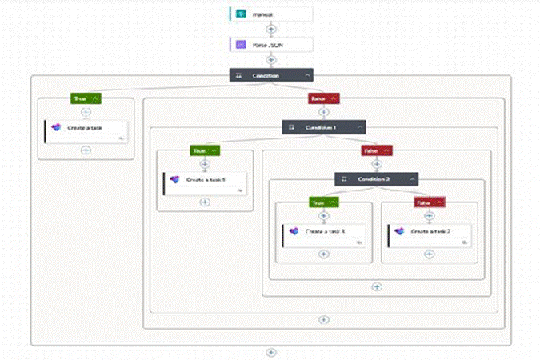
\includegraphics[width=0.52\textwidth,max width=\textwidth]{images/image53.png}
  \caption{Agent 3 Power Automate Flow Logic}
  \label{fig:image53}
\end{figure}

\begin{center}\small\textbf{Listing: Step 6: Power Automate dispatch loop with rate-limit delay (updating.py)}\end{center}
\begin{Verbatim}[breaklines=true,fontsize=\footnotesize,frame=single]
for _, row in tasks_df.iterrows():
payload = {
"PF":
row["PF"],
"PC":
row["PC"],
"request_type": row["request_type"],
"assigned_to":
row["assigned_to"],
"priority":
row["priority"],
"deadline":
row["deadline"],
}
r = requests.post(AGENT3_FLOW_URL, json=payload, verify=False)
if r.status_code not in (200, 202):
print(f"[WARN] Row {row['PC']}: flow returned {r.status_code}")
time.sleep(2)
# mandatory M365 tenant rate limit
\end{Verbatim}

\subsection{Desktop Interface}

Agent 3 is operated through a standalone Python tkinter application (updating UI.py). This design reflects a practical constraint: the Pilot must browse the local filesystem for three input files that may be 50--200 MB each. Figure 4.19 shows the interface in its pre-execution state. The "Dernier consultant affecté" dropdown records the last consultant assigned in the previous run, maintaining the round-robin state across daily executions.

\begin{figure}[H]
  \centering
  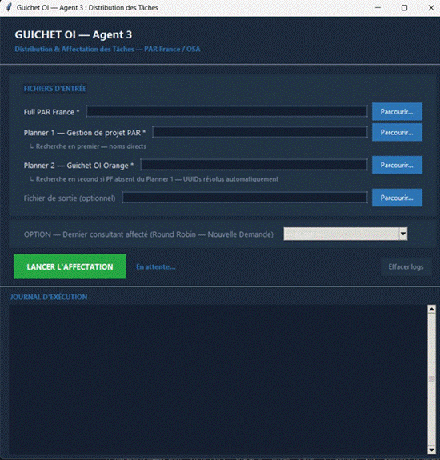
\includegraphics[width=0.52\textwidth,max width=\textwidth]{images/image54.png}
  \caption{Guichet OI Agent 3 desktop UI with file inputs, configuration controls, and execution journal.}
  \label{fig:image54}
\end{figure}

\section{Platform Integration and Local Development Validation}

The Unified Platform frontend (guichet-oi-platform) was served locally throughout the SENTINEL Fleet validation period using ng serve. Figure 4.20 shows the build output: the initial bundle totals 106.54 kB (main.js 105.27 kB, styles.css 1.18 kB, polyfills.js 95 bytes), produced in 10.258 seconds. The platform was accessible at http://localhost:4200/ for all agent control operations during testing.

\begin{figure}[H]
  \centering
  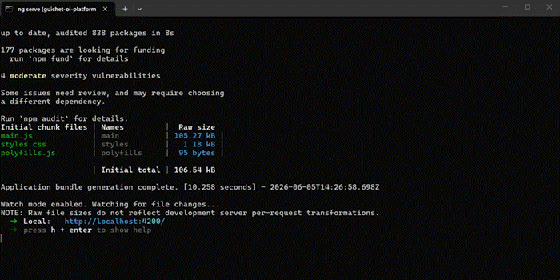
\includegraphics[width=0.52\textwidth,max width=\textwidth]{images/image55.png}
  \caption{Angular Platform Local Build: ng serve Bundle Output}
  \label{fig:image55}
\end{figure}

\section{System Validation and Performance Results}

Validation was conducted over two weeks against the live Orange Exchange environment, production SharePoint SUIVI list, and production Planner boards. Results are measured against the non-functional requirements defined in Chapter 3 \S{}3.1.2.

\begin{table}[H]
  \centering
  \caption{Fleet-level performance results against Chapter 3 \S{}3.1.2 targets}
  \renewcommand{\arraystretch}{1.0}
  \footnotesize
  \begin{tabularx}{\textwidth}{|>{\raggedright\arraybackslash}p{2.3cm}|X|X|X|X|}
    \hline
    \textbf{Agent} & \textbf{Workflow} & \textbf{Pre-automation} & \textbf{Post-automation} & \textbf{Reduction} \\ \hline
    Agent 1 & POI validation & 15--20 min/email $\times$ \textasciitilde{}15/day & \textless{} 60 s/email & \textasciitilde{}95\% \\ \hline
    Agent 2 & CAFF returns & Variable 1-day KPI missed & \textless{} 60 s/return & KPI closed \\ \hline
    Agent 3 & Task distribution & 30--45 min/batch & \textasciitilde{}2 min pipeline + \textasciitilde{}4 min dispatch & \textasciitilde{}95\% \\ \hline
  \end{tabularx}
\end{table}

Agent 1 median end-to-end latency (email receipt in FINOI to Power Automate HTTP 202) was 43 seconds, within the 90-second target. The dominant cost is EWS connection establishment (8--12 seconds) and the corporate proxy round-trip. The Power Automate webhook accounts for approximately 4--7 seconds. Agent 2 achieved equivalent latency. The one-working-day KPI was met on every validation run: CAFF return to Planner task creation with consultant assignment never exceeded 60 seconds.

Agent 3 pipeline phase (Steps 1--5, pandas processing through workbook generation) completed in 1 minute 47 seconds median for a 112-row batch. Dispatch phase (Step 6, 112 webhooks at 2-second intervals) completed in 3 minutes 42 seconds. Total time: 5 minutes 29 seconds. The Pilot daily time investment was reduced from 30--45 minutes to the time required to select three files and review the output workbook.

\section*{Conclusion}
\addcontentsline{toc}{section}{Conclusion}

This chapter has documented the complete implementation of the SENTINEL Automation Fleet at the source-code level. The six Python files email\_listener.py, updatePOI.py, updateretour.py, updating.py, Extract uuids.py, and uuid\_map.json constitute the entire automation layer. No commercial RPA platform, no browser driver, and no cloud AI service is involved. Every processing decision is deterministic, logged, and auditable.

Three implementation details proved critical and are worth retaining for future maintainers. First, the PC regex fix: the initial \textbackslash{}\textbackslash{}d+ pattern silently truncated alphanumeric codes; replacing it with [\textasciicircum{}\#\textbackslash{}\textbackslash{}s]+ resolved the issue without any other code change. Second, the NO\_PROXY environment variable: without it, Power Automate webhook calls are blocked by the Orange proxy with HTTP 403 a constraint invisible during development on a non-proxied network. Third, the NoVerifyHTTPAdapter: Orange Exchange uses a self-signed certificate that standard Python requests will reject; the adapter suppresses this check while keeping all other TLS properties intact.

The Guichet OI Automation Platform, whose local build and agent control interfaces were validated in this chapter, serves as the operational surface for all three agents in production. Its full implementation Spring Boot backend, JWT authentication, audit trail, and Azure deployment is documented in Chapter 6. The following chapter presents the FiberGate AI Service, which addresses the document understanding dimension of the OSA workflow through a LayoutLMv3 transformer fine-tuned on an in-house annotated corpus.
